\documentclass[twocolumn,a4j]{jsarticle}
\setlength{\topmargin}{-18.5cm}
\setlength{\oddsidemargin}{-8.5mm}
\setlength{\evensidemargin}{-8.5mm}
\setlength{\textwidth}{19cm}
\setlength{\textheight}{26.5cm}

\usepackage[top=15truemm,bottom=20truemm,left=20truemm,right=20truemm]{geometry}
\usepackage[latin1]{inputenc}
\usepackage{amsmath}
\usepackage{amsfonts}
\usepackage{amssymb}
\usepackage[dvipdfmx]{graphicx}
\usepackage[hang,small,bf]{caption}
\usepackage[subrefformat=parens]{subcaption}
\usepackage[dvipdfmx]{color}
\usepackage{listings}
\usepackage{listings,jvlisting}
\usepackage{geometry}
\usepackage{framed}
\usepackage{color}
\usepackage[dvipdfmx]{hyperref}
\usepackage{ascmac}
\usepackage{enumerate}
\usepackage{tabularx}
\usepackage{cancel}
\usepackage{scalefnt}
\usepackage{overcite}
\usepackage{otf}
\usepackage{multicol}
\usepackage[geometry]{ifsym}

\renewcommand{\figurename}{Fig.}
\renewcommand{\tablename}{Table }

\hypersetup{%
    hidelinks %リンクの色消し
}

\lstset{
basicstyle={\ttfamily},
identifierstyle={\small},
commentstyle={\smallitshape},
keywordstyle={\small\bfseries},
ndkeywordstyle={\small},
stringstyle={\small\ttfamily},
frame={tb},
breaklines=true,
columns=[l]{fullflexible},
xrightmargin=0zw,
xleftmargin=3zw,
numberstyle={\scriptsize},
stepnumber=1,
numbersep=1zw,
lineskip=-0.5ex
}

% キャプション後ろのダブルコロンを消す
\makeatletter
\long\def\@makecaption#1#2{%
  \vskip\abovecaptionskip
  \iftdir\sbox\@tempboxa{#1\hskip1zw#2}%
    \else\sbox\@tempboxa{#1 #2}%
  \fi
  \ifdim \wd\@tempboxa >\hsize
    \iftdir #1\hskip1zw#2\relax\par
      \else #1 #2\relax\par\fi
  \else
    \global \@minipagefalse
    \hbox to\hsize{\hfil\box\@tempboxa\hfil}%
  \fi
  \vskip\belowcaptionskip}
\makeatother


\makeatletter
\def\@maketitle
{
\begin{center}
{\LARGE \@title \par}
\end{center}
\begin{flushright}
{\large \@date}\\
{\large 京都工芸繊維大学 大学院 機械設計学専攻 計測システム工学研究室}\\
{\large M2 \@author}
\end{flushright}
\par\vskip 1.5em
}
\makeatother

\author{来代 勝胤 / KITADAI Masatsugu}
\title{令和5年度 10月度 月例報告書}
\date{2023/10/23}


\begin{document}
\columnseprule=0.1mm
\maketitle

\section*{報告内容}
\begin{enumerate}[1.]
	\item 二次流れの計測手法の概要
	\item 粒子位置の特定
	\item 粒子のクラスタリング
	\item クラスタマッチング
	\item 二次流れの解析結果
	\item 11月の予定
\end{enumerate}

\section*{進捗報告}
今月は,局所的な流れに対応した二次流れ解析の実現に向けて
解析手法の検討を行った.そこで,同一粒子の粒子像から構成される粒子クラスタを取得し,
その情報を用いた粒子追跡アルゴリズムを作成した.
その結果,これまで解析できていなかった車両モデルの流れ場について,
流れ構造を確認することができた.

\section{概要:二次流れの解析手法}
はじめに,本研究の目的及び二次流れの計測手法について説明する.
本研究では,二次流れの定量的な流れ場及び時刻変化の取得を目的に,
計測手法の開発に取り組んできた.
また,計測対象となる”二次流れ”とは主流方向に垂直な面内に発生する流れのことを指す.

\subsection{計測手法}
\begin{figure}[htbp]
	\centering
	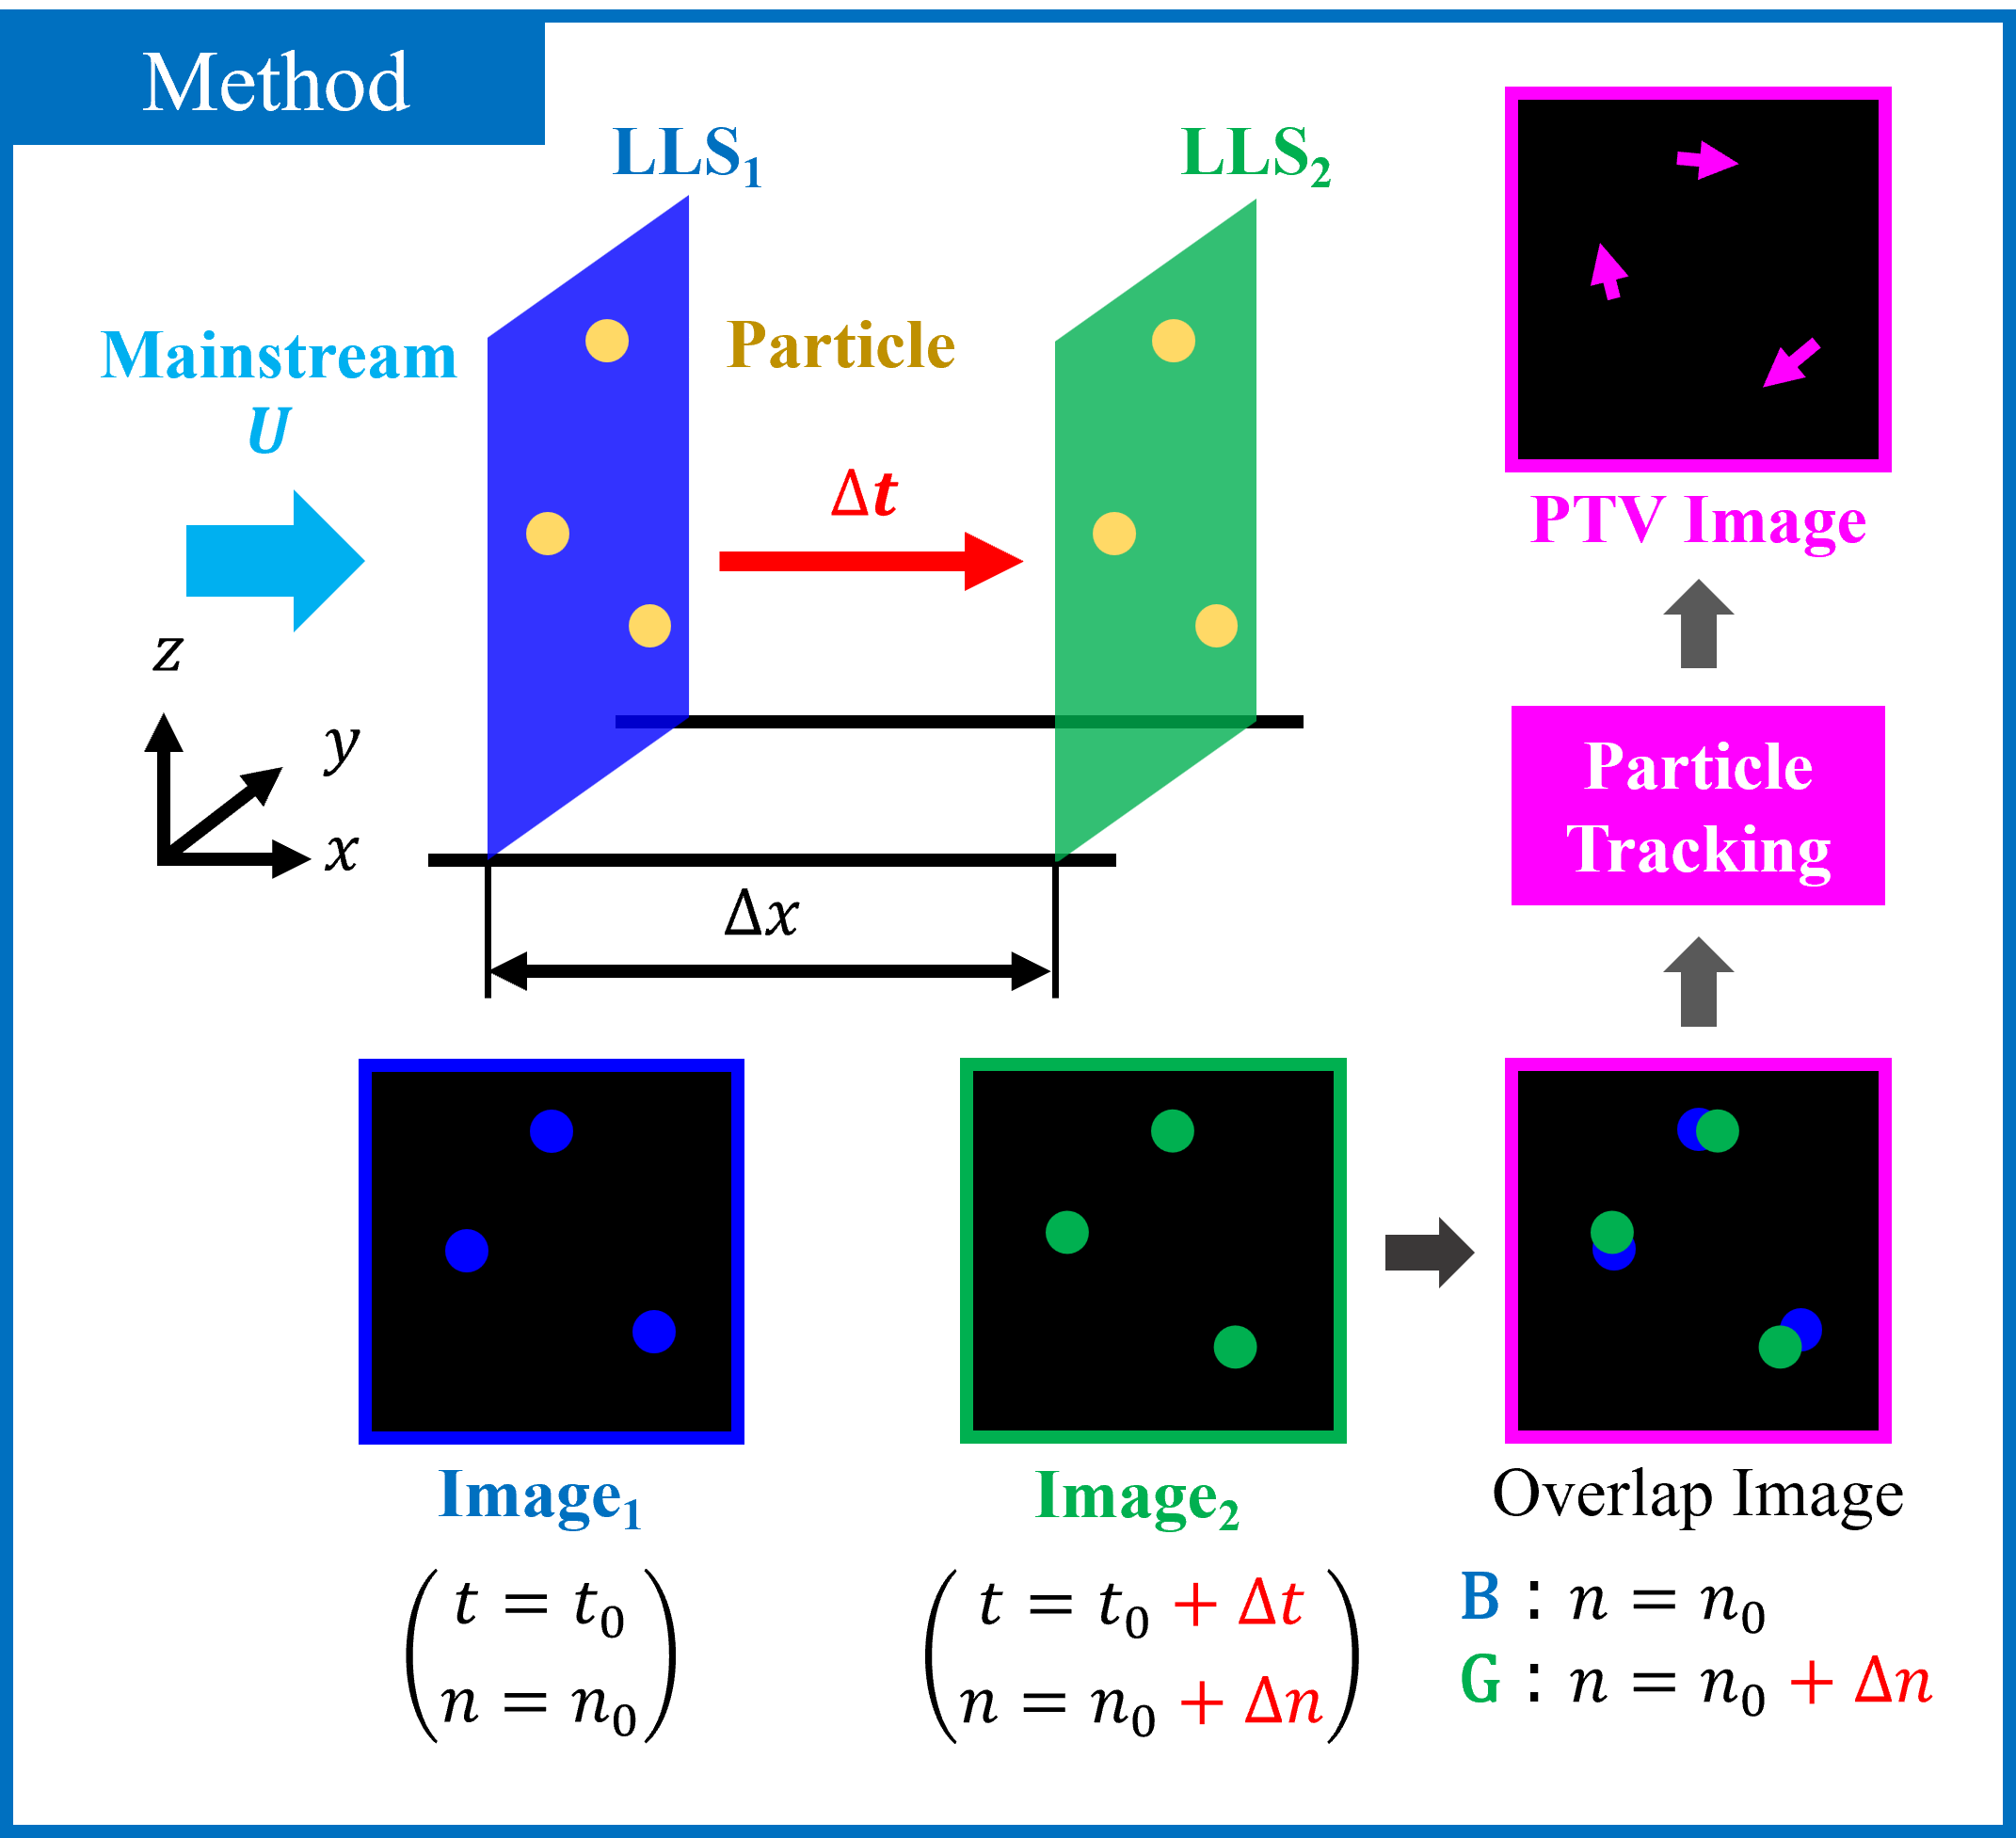
\includegraphics[keepaspectratio, width=80mm]{../images/method.png}
	\caption{PTV method for secondary flow analysis}
\end{figure}

\newpage
ここで,計測手法の概略図を Fig.1 に示す.
図内では,紙面の左側から右側に向かって主流方向が流れていることを想定し,
その主流に対して垂直に異なる色の2枚のレーザーシートを,微小間隔 $\Delta x$ を持って設置する.
前方のレーザーシート LLS$_1$ および,後方のレーザーシート LLS$_2$を通過する粒子を
高速度カラーカメラを用いて撮影し,その時刻差 $\Delta t$ に対応させて撮影画像を解析することで
垂直な平面内の流れ場を得るという計測手法である.

\subsection{実験装置}

FIg.2 に実際に使用している実験装置の概略図を示す.
本研究では,海流水槽内に設置したモデル周りの流れ場に対して,
青・緑のレーザービーム装置2台を用いて流れ場の撮影を行う.
また,凹レンズを用いてレーザーシートを作成し,
ミラーによってその間隔を調整できるシステムになっている.
ここで,流れ構造は主流校からの撮影ができないため,
水・空気間の屈折を防ぐ水槽を通して,斜め後方からの撮影となる.

\begin{figure}[htbp]
	\centering
	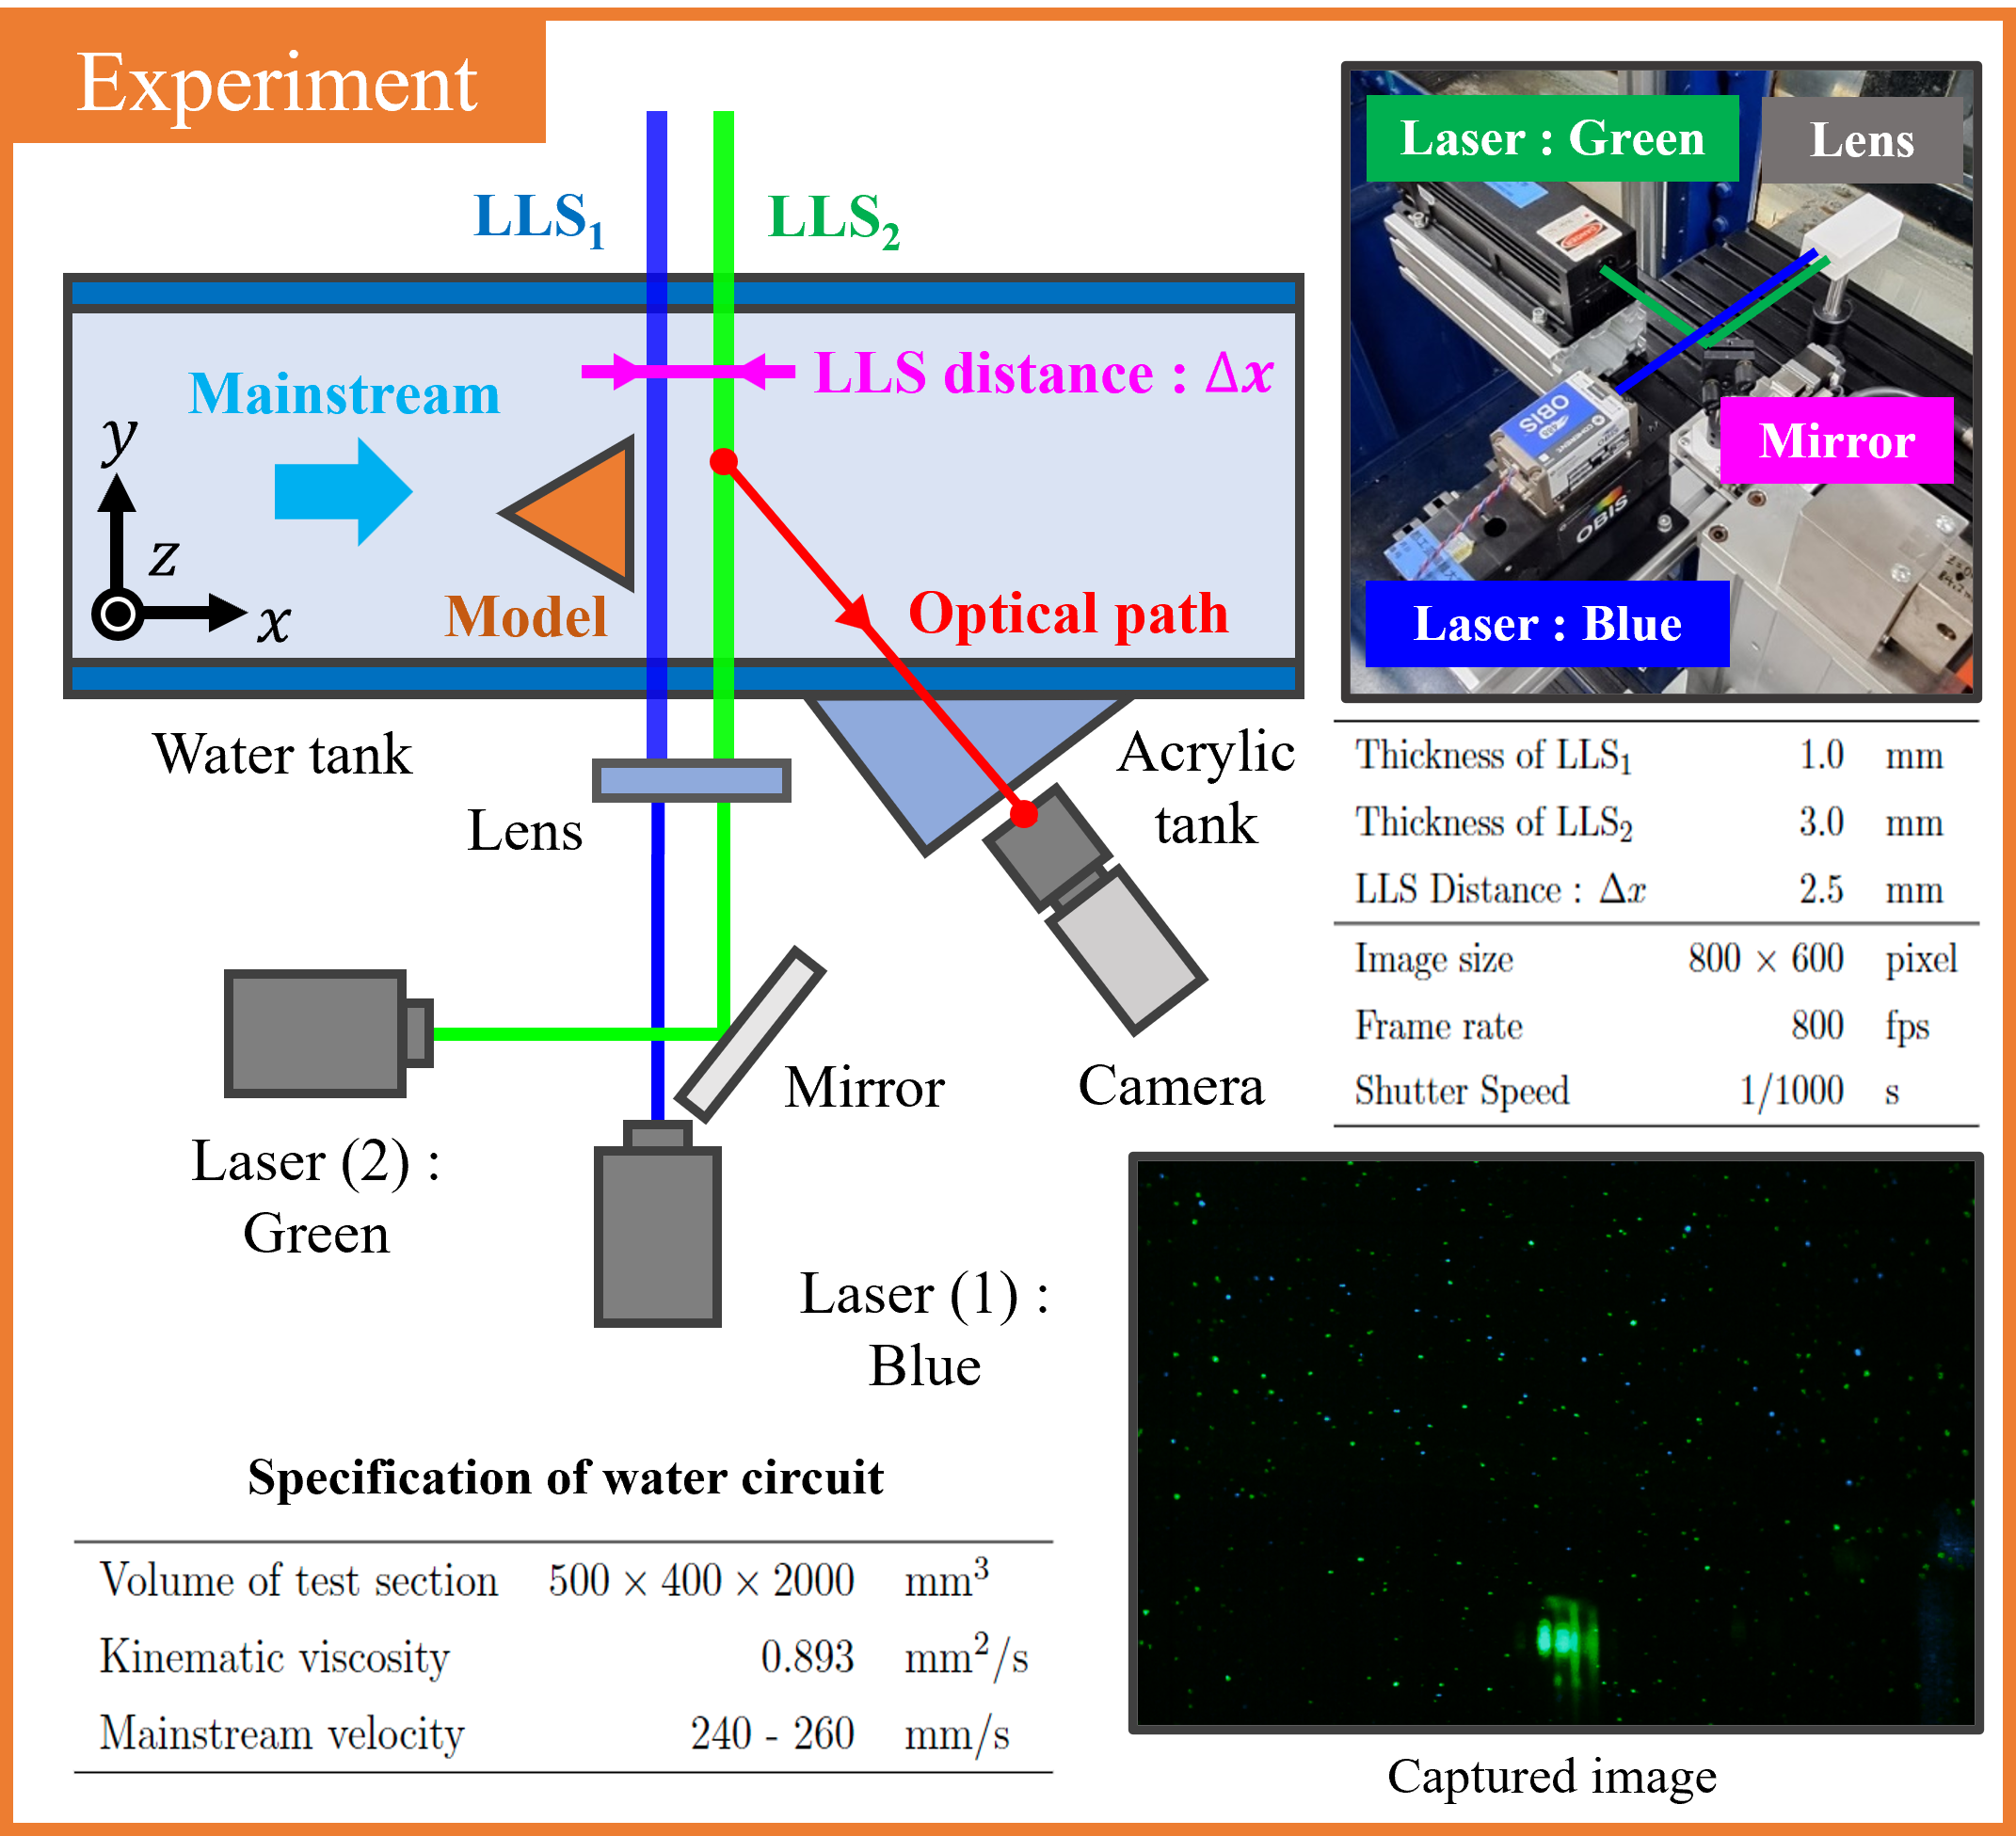
\includegraphics[keepaspectratio, width=80mm]{../images/experiment.png}
	\caption{Experiment setup}
\end{figure}

\newpage
\subsection{粒子追跡手法}
次に,粒子追跡法を応用した流れ場の解析手法について説明する.
今回の解析では,Table 1 の条件で行っていることを前提とする.
また,レーザーシートの配置条件から,
青色のレーザーシートを通過した後に緑色のレーザーシートを通過することがわかっている.
\begin{table}[hbtp]
	\centering
	\caption{Condition of capturing images}
	\begin{tabular}{l c c}
		\hline
		Shutter speed & 1/1000 & [s]   \\ \hline
		Frame rate    & 800    & [fps] \\ \hline
	\end{tabular}
\end{table}

ここで,レーザーシートに一定の厚みがあることから,
同一の粒子は複数枚の画像に映り込む.
また,撮影が斜め後方からの撮影により,
粒子像は下流に向かうにつれて,画像の左から右へとスライドする.
そこで,各色の粒子像について同一の粒子からなる粒子像をクラスタリングから判別する.
また,画像横方向のスライドによる粒子像の移動量の情報を,
クラスタどうしのマッチングに利用することで粒子追跡を行い,
流れ場を解析することを検討した.

\begin{figure}[htbp]
	\centering
	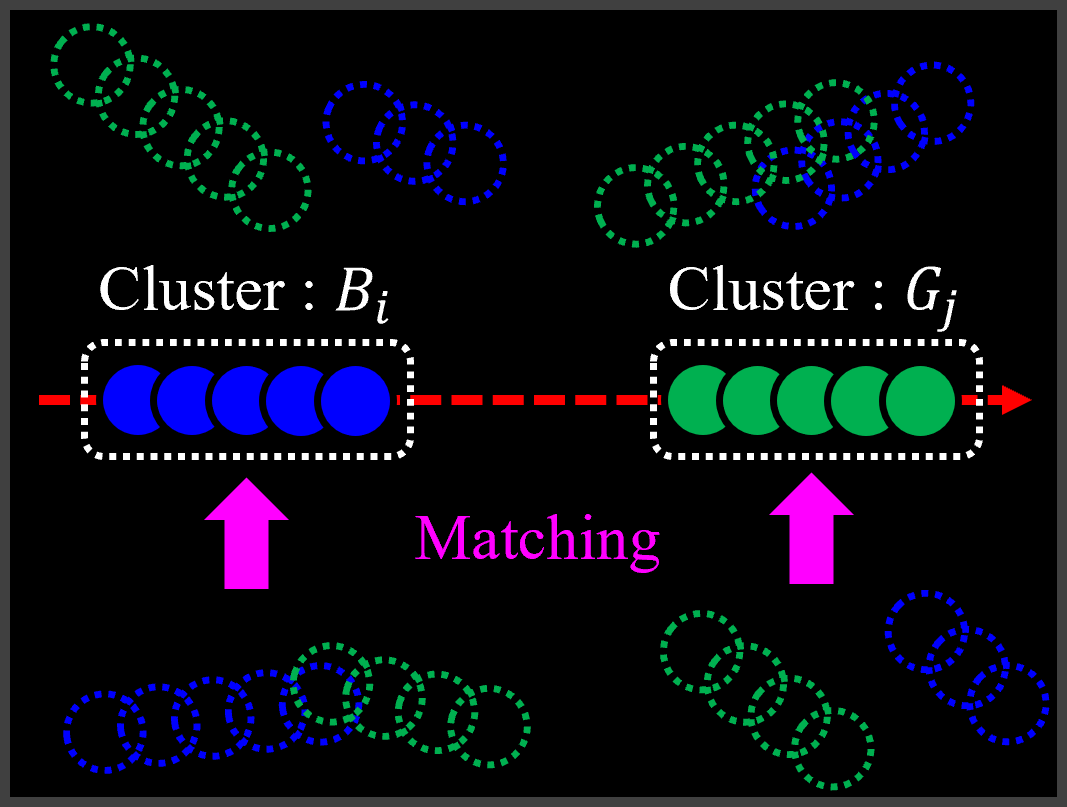
\includegraphics[keepaspectratio, width=70mm]{../images/PTV_mthod_with_cluster_matching.png}
	\caption{PTV with cluster matching}
\end{figure}

\section{粒子位置の特定}
はじめに粒子位置の特定について,その手法と結果を示す.
撮影画像は,背景処理を施した後,粒子マスク相関法を用いて
画像内に含まれる粒子の中心位置を検出する,
Fig.4に粒子マスクとの相関係数を示した結果,Fig.5に特定した粒子位置の結果について示す.
粒子マスク相関法を用いることで,輝度値の低い粒子でも検出することができる.

\newpage
\begin{figure}[htbp]
	\centering
	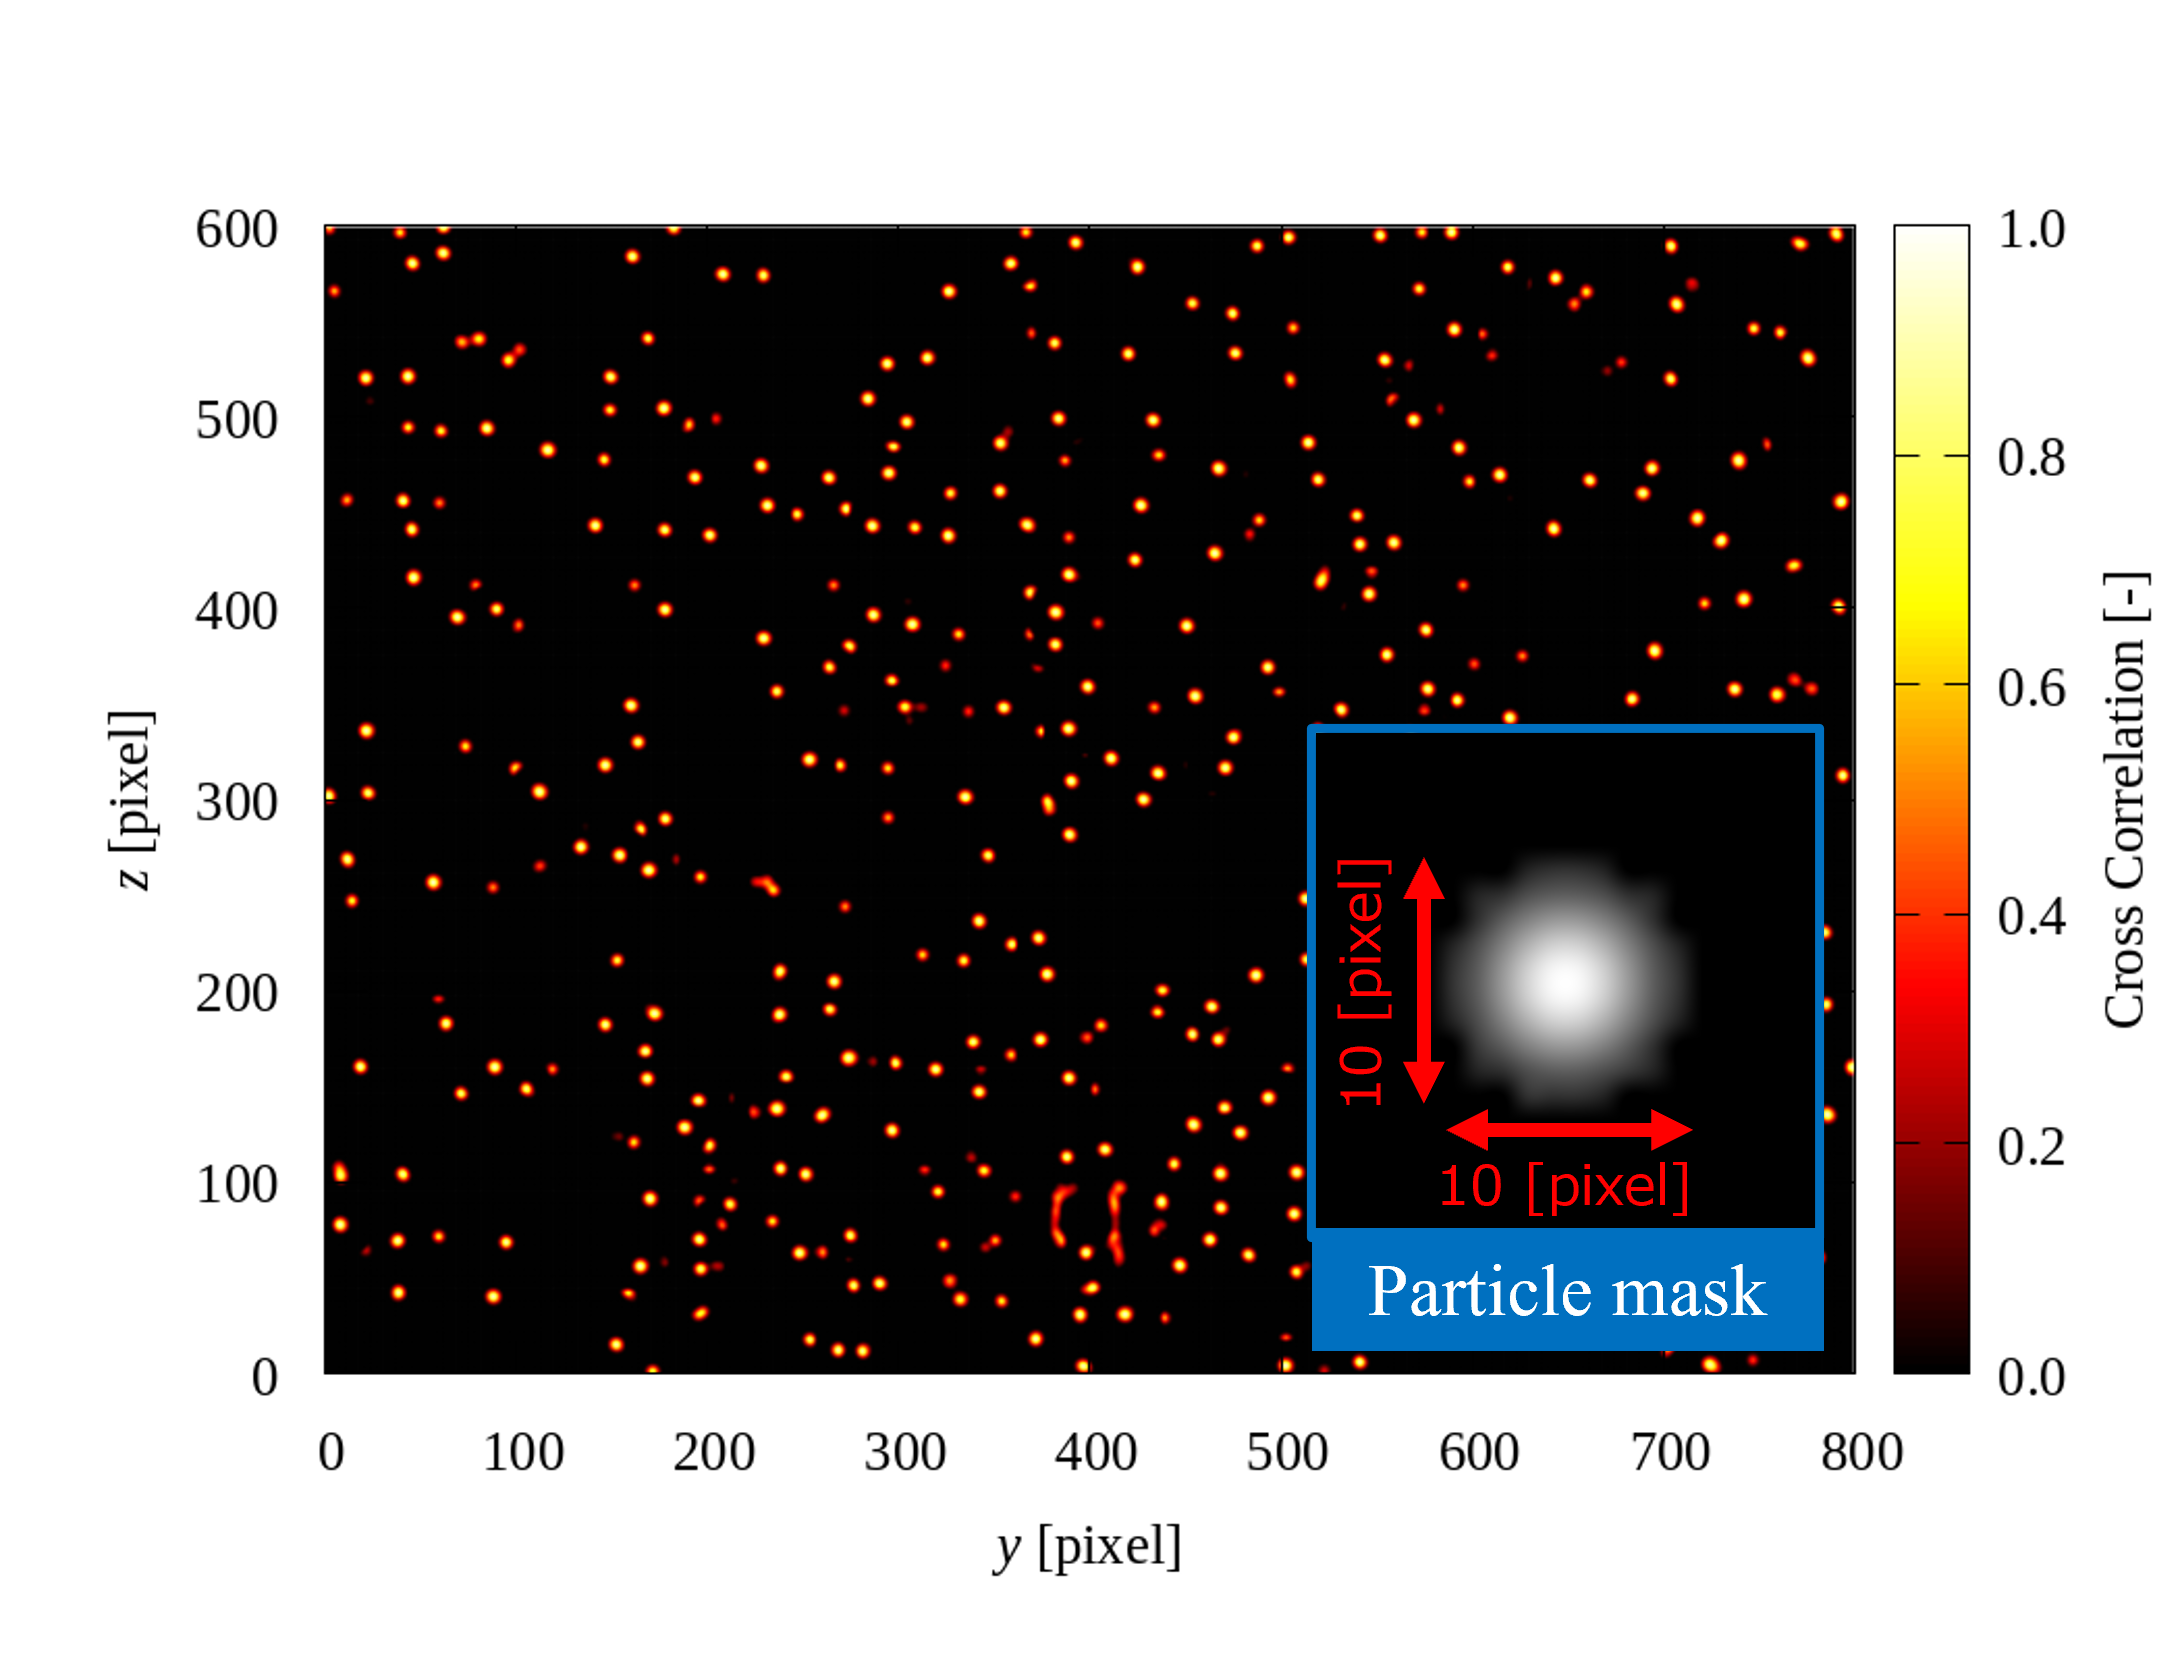
\includegraphics[keepaspectratio, width=80mm]{../images/closs-correlation_for_particle.png}
	\caption{Cross-correlation for particle image}
	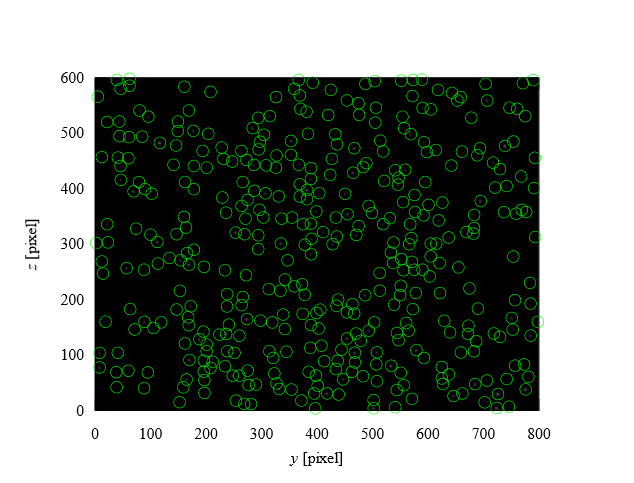
\includegraphics[keepaspectratio, width=80mm]{../images/particle_position.png}
	\caption{Particle position for green image}
\end{figure}

\section{粒子のクラスタリング}
次に,粒子のクラスタリングについて説明する.
クラスタリングは,同一の粒子が複数枚の撮影画像に映り込む特徴から
その粒子の軌道を特定し,粒子追跡の情報として使用する.

\begin{figure}[htbp]
	\centering
	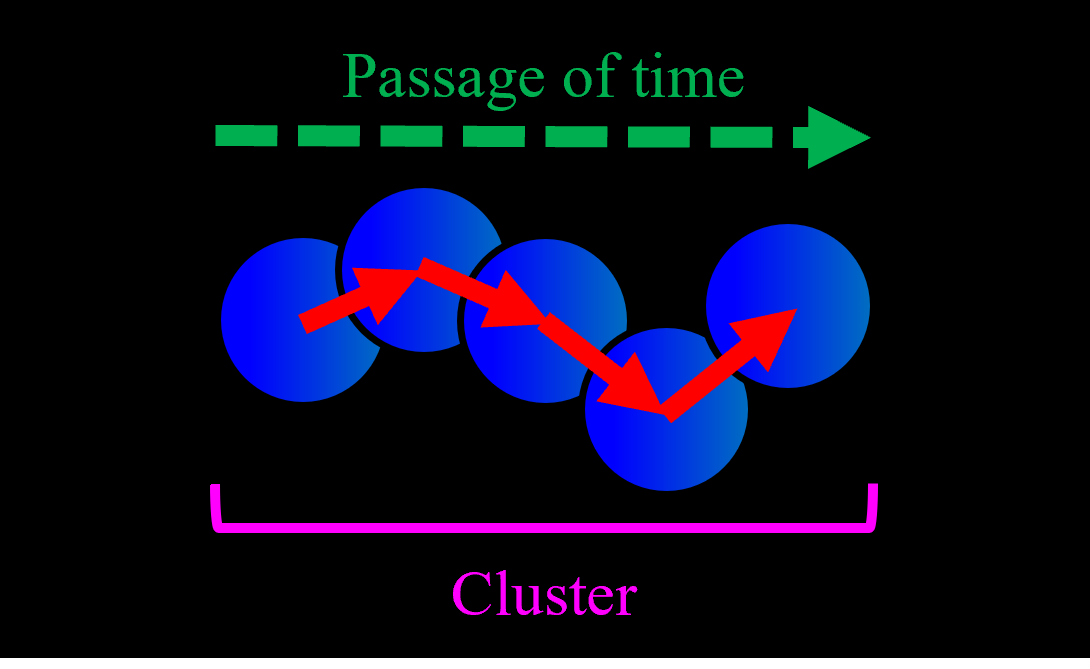
\includegraphics[keepaspectratio, width=50mm]{../images/how_to_get_cluster.png}
	\caption{PTV for clustering}
\end{figure}

ここで,クラスタリングの手法として,Fig.6に示すように,
時刻の移動に粒子の移動を最近法を用いて追跡し,
対応が取れなくなった時点で,それを一つのクラスタとして取得する.
実際に,クラスタリングを行った結果を Fig.7 に示す.
この画像内における,点が粒子位置,それをつなぐ線分が一つのクラスタを示している.

\begin{figure}[htbp]
	\centering
	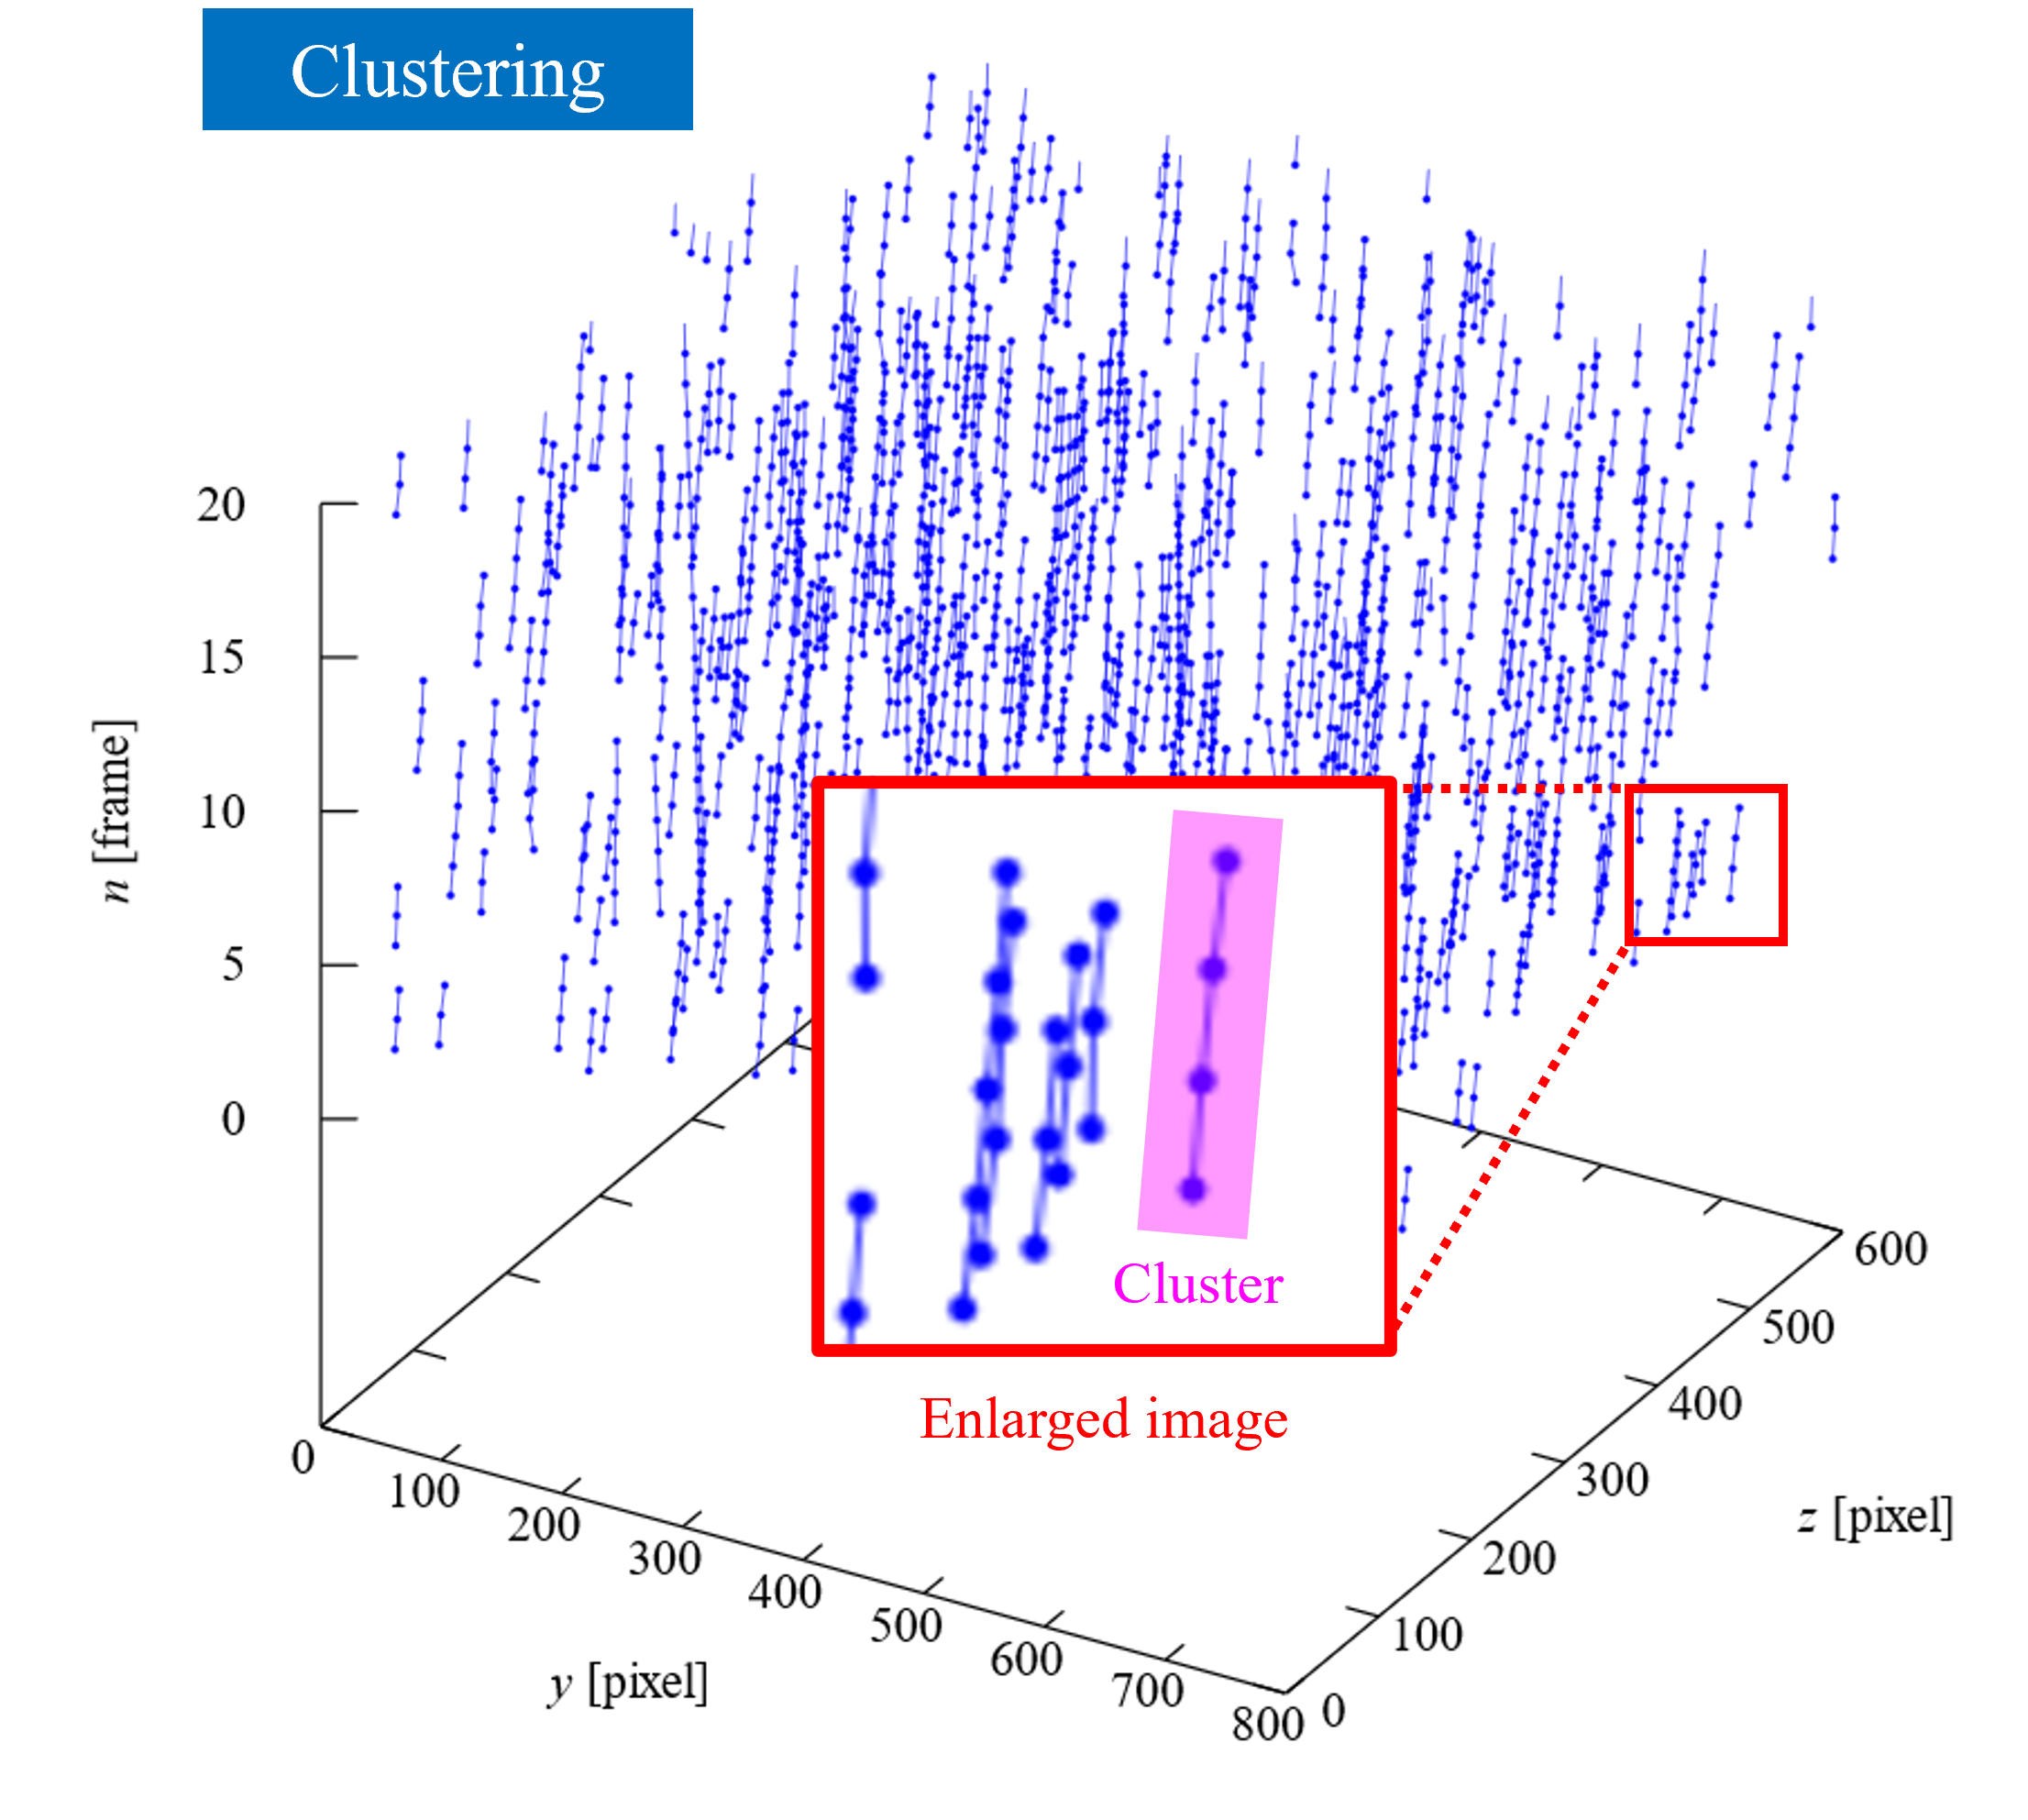
\includegraphics[keepaspectratio, width=75mm]{../images/clustering_for_blue_image.png}
	\caption{Clustering for blue image}
\end{figure}

\section{クラスタマッチング}
作成したクラスタを用いて粒子追跡を行う.
ここで,粒子追跡を行うためには,クラスタどうしのマッチングを行う必要がある.
マッチングは,それぞれのクラスタから得られる近似直線の傾きと
それを用いて計算される予測点及び,クラスタ中心との距離を用いて行う.\\

\subsubsection*{$\blacksquare$ クラスタ中心}
\begin{eqnarray*}
	y'_i &=& \frac{1}{N_i} \sum_{j=1}^{N} y_{ij} \\
	z'_i &=& \frac{1}{N_i} \sum_{j=1}^{N} z_{ij} \\
	n'_i &=& \frac{1}{N_i} \sum_{j=1}^{N} n_{ij} \\
	i &:& \text{クラスタ番号}\\
	j &:& \text{フレーム番号}\\
	N_i &:& i \text{番目の粒子のフレーム総数}
\end{eqnarray*}

\subsubsection*{$\blacksquare$ 主流方向速度の推定}
\begin{eqnarray*}
	u_i &=& T \times \frac{f}{N_i}\\
	T_b &:& \text{青色レーザーシート厚み} \\
	f &:& \text{フレームレート}\\
\end{eqnarray*}

\newpage
実際に,粒子クラスタどうしをマッチングさせた結果を Fig.8, 9 に示す.
この画像から,青の粒子クラスタの延長線上に
緑の粒子クラスターが存在することがわかり,正しく追跡が行われていると考えられる.

\begin{figure}[htbp]
	\centering
	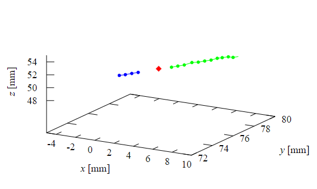
\includegraphics[keepaspectratio, width=65mm]{../images/cluster_matching_1.png}
	\caption{Cluster matching : 3D view}
	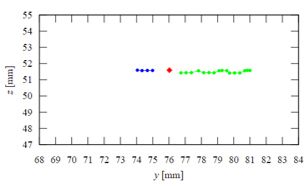
\includegraphics[keepaspectratio, width=65mm]{../images/cluster_matching_2.png}
	\caption{Cluster matching : $y-z$ view}
\end{figure}

\section{二次流れの解析結果}
次に,これまでの粒子追跡方を用いて得られた二次流れの解析結果を示す.
ここでは,Fig.10に示す三角翼モデルとFig.11に示す車両モデルを用いた計測結果について示す.\\

\subsection{計測用モデル}
\begin{figure}[htbp]
	\centering
	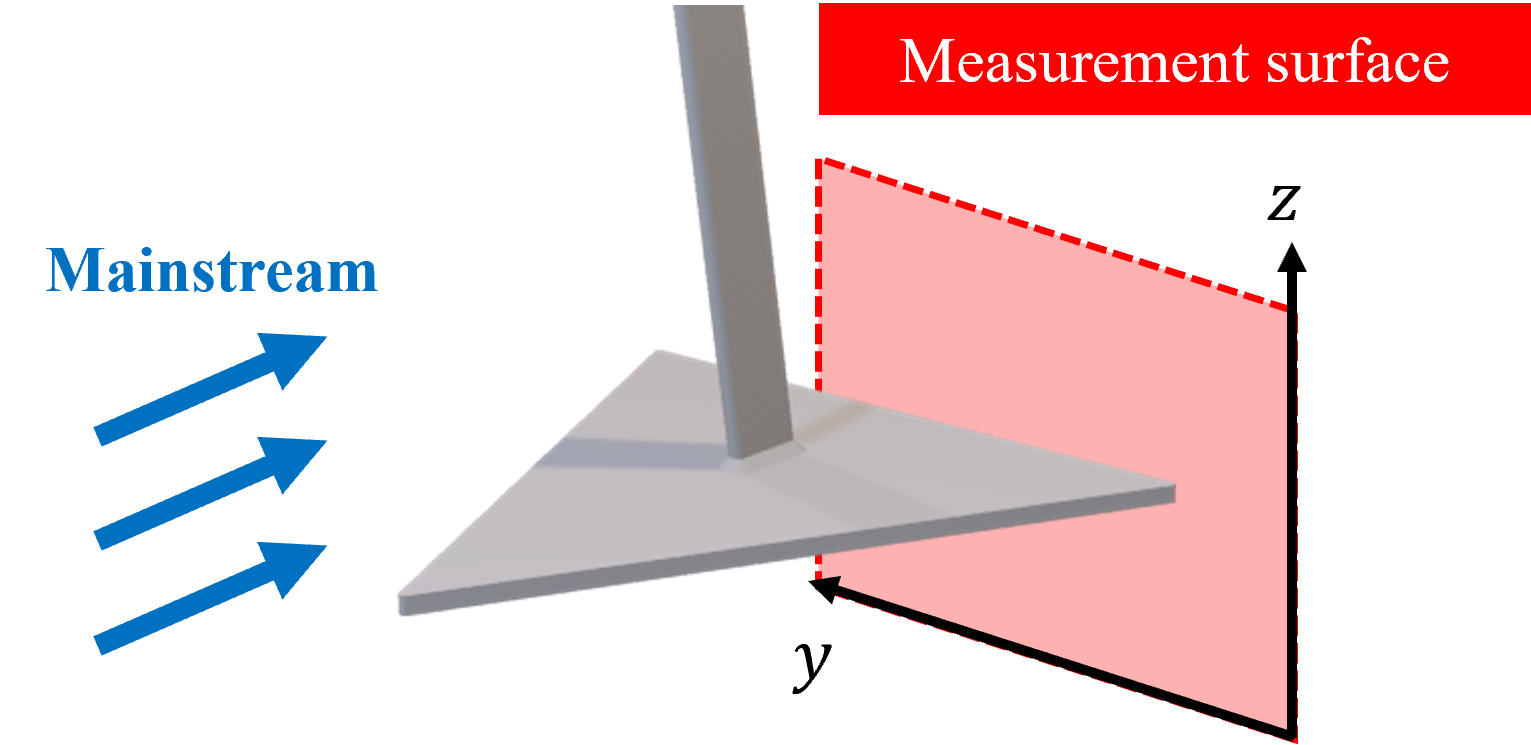
\includegraphics[keepaspectratio, width=60mm]{../images/delta_wing_model.png}
	\caption{Delta wing model}
	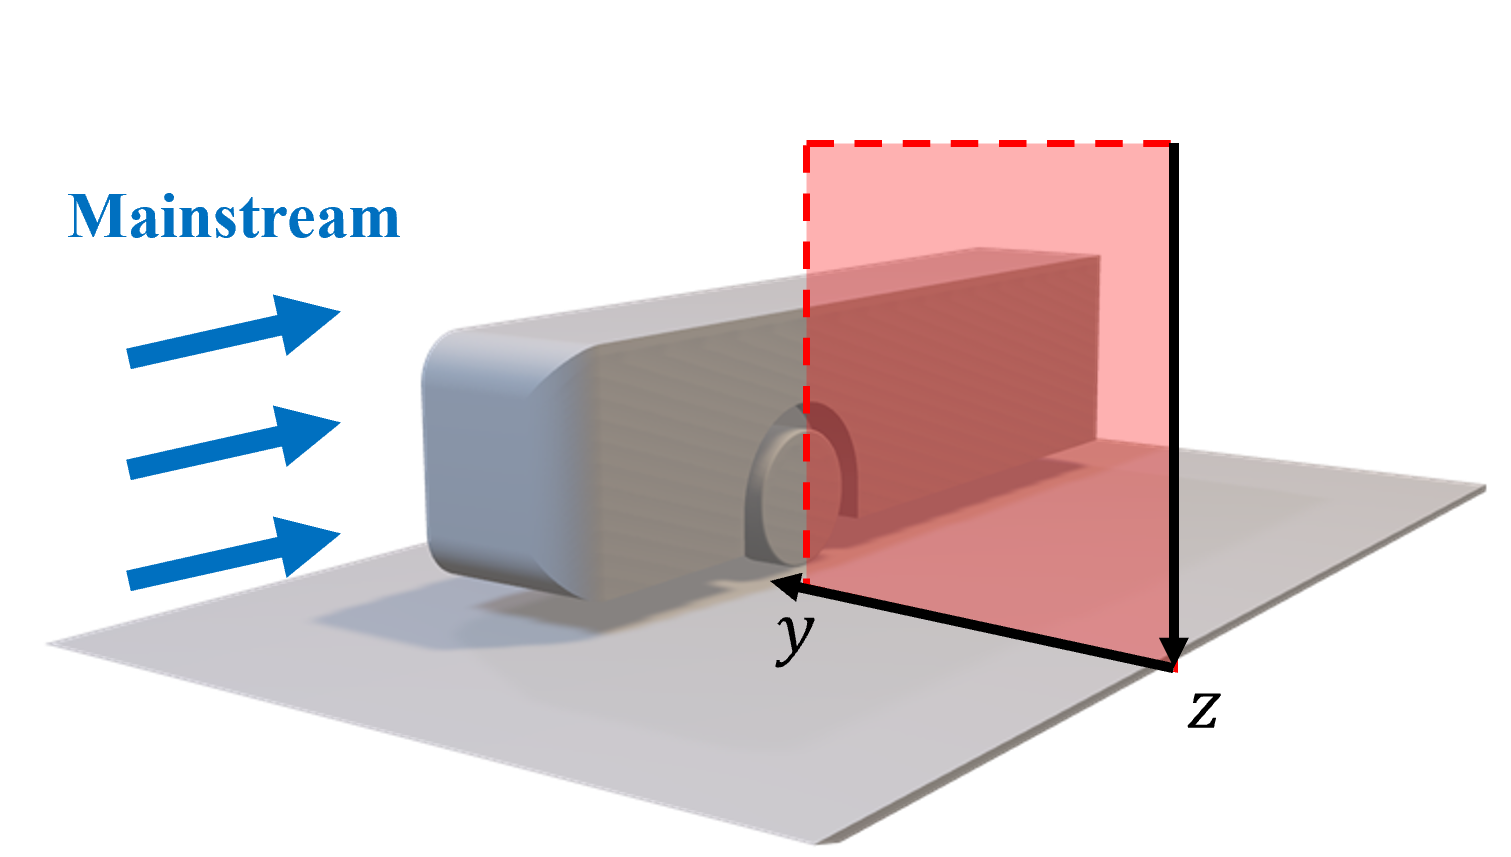
\includegraphics[keepaspectratio, width=60mm]{../images/vehicle_model.png}
	\caption{Vehicle model}
\end{figure}

\newpage
\subsection{三角翼:右翼後流}
三角翼後流の計測について,Fig.12に解析結果を示す.
これまでの結果と同様に翼端に反時計回りの渦構造を確認することができる.
このことから,粒子クラスタマッチングが正しく機能していることを確認することができる.

\begin{figure}[htbp]
	\centering
	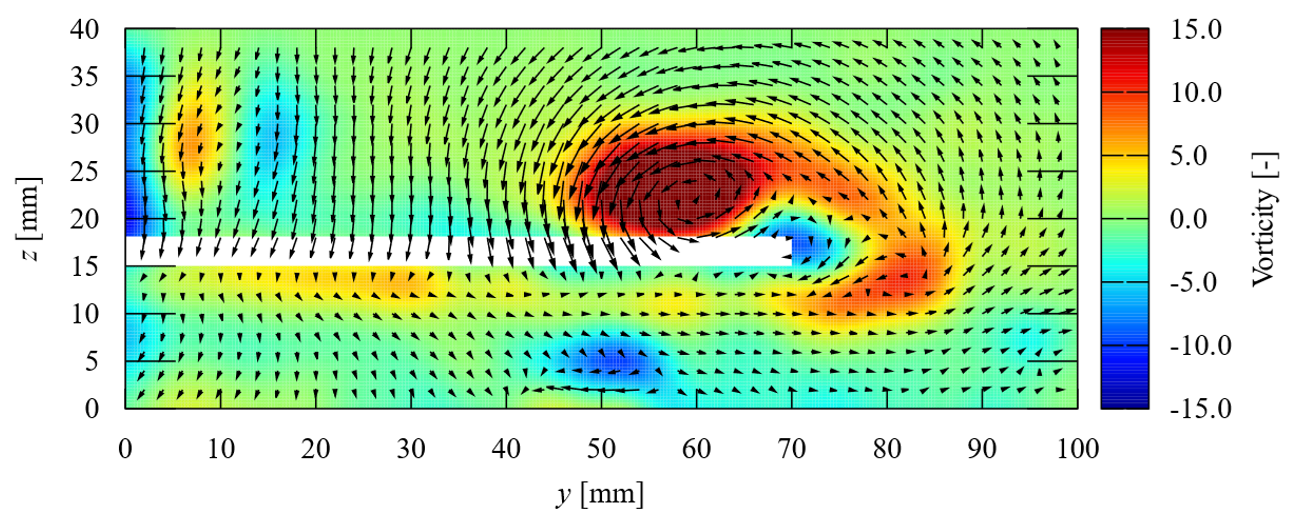
\includegraphics[keepaspectratio, width=82mm]{../images/delta_wing.png}
	\caption{PTV :Wake of delta wing}
\end{figure}

\subsection{車両モデルの測定}
車両モデルについては,タイヤの回転の有無を比較するために,計測を行った.
Fig.13にタイヤ回転無しの計測結果,およびFig.14にタイヤ回転有りの計測結果を示す.
解析結果から,これまで確認できていなかった
地面板とタイヤモデルの接地部に発生する渦構造を確認することができた.

\begin{figure}[htbp]
	\centering
	\includegraphics[keepaspectratio, width=82mm]{../images/vehicle_stop.png}
	\caption{PTV : Vehicle model without tire rotation}
	\baselineskip 4mm
	\includegraphics[keepaspectratio, width=82mm]{../images/vehicle_rolling.png}
	\caption{PTV Measurement :Vehicle model with tire rotation}
\end{figure}

\section{11月の予定}
\begin{itemize}
	\item 車両モデルの計測
	\item 数値シミュレーションによる性能評価
\end{itemize}

\newpage
$\blacksquare$ コサイン類似度
\begin{eqnarray*}
	cos(\theta) &=& \frac{\vec{a} \cdot \vec{b}}{|\vec{a}| |\vec{b}|} \\
\end{eqnarray*}

\end{document}